%	PACKAGES AND OTHER DOCUMENT CONFIGURATIONS

\documentclass[11pt, a4paper,twocolumn]{article} % 10pt font size (11 and 12 also possible), A4 paper (letterpaper for US letter) and two column layout (remove for one column) Use additional titlepage argument to generate this
%\documentclass[12pt, a4paper,twocolumn,titlepage]{article}

%%%%%%%%%%%%%%%%%%%%%%%%%%%%%%%%%%%%%%%%%
% Wenneker Article
% Structure Specification File
% Version 1.0 (28/2/17)
%
% This file originates from:
% http://www.LaTeXTemplates.com
%
% Authors:
% Frits Wenneker
% Vel (vel@LaTeXTemplates.com)
%
% License:
% CC BY-NC-SA 3.0 (http://creativecommons.org/licenses/by-nc-sa/3.0/)
%
%%%%%%%%%%%%%%%%%%%%%%%%%%%%%%%%%%%%%%%%%

%----------------------------------------------------------------------------------------
%	PACKAGES AND OTHER DOCUMENT CONFIGURATIONS
%----------------------------------------------------------------------------------------

\usepackage[english]{babel} % English language hyphenation

\usepackage{microtype} % Better typography

\usepackage{verbatim} % Allows mulitline commenting

\usepackage{amsmath,amsfonts,amsthm} % Math packages for equations

\usepackage[svgnames]{xcolor} % Enabling colors by their 'svgnames'

\usepackage[hang, small, labelfont=bf, up, textfont=it]{caption} % Custom captions under/above tables and figures

\usepackage{subcaption}

\usepackage{booktabs} % Horizontal rules in tables

\usepackage{lastpage} % Used to determine the number of pages in the document (for "Page X of Total")

\usepackage{graphicx} % Required for adding images

\usepackage{enumitem} % Required for customising lists
\setlist{noitemsep} % Remove spacing between bullet/numbered list elements

\usepackage{sectsty} % Enables custom section titles
\allsectionsfont{\usefont{OT1}{phv}{b}{n}} % Change the font of all section commands (Helvetica)

\usepackage{bm} % Used for bold font in math environments

\usepackage{siunitx} % Used for SI units

\usepackage{tikz} % Used for tikz diagrams
\usetikzlibrary{calc} % Enable math in tikz code

\newcommand*{\subscript}[1]{\ensuremath{_\textrm{{\scriptsize #1}}}}  %Non italic subscripts

%----------------------------------------------------------------------------------------
%	MARGINS AND SPACING
%----------------------------------------------------------------------------------------

\usepackage{geometry} % Required for adjusting page dimensions

\geometry{
	top=1cm, % Top margin
	bottom=1.5cm, % Bottom margin
	left=2cm, % Left margin
	right=2cm, % Right margin
	includehead, % Include space for a header
	includefoot, % Include space for a footer
	%showframe, % Uncomment to show how the type block is set on the page
}

\setlength{\columnsep}{7mm} % Column separation width

%----------------------------------------------------------------------------------------
%	FONTS
%----------------------------------------------------------------------------------------

\usepackage[T1]{fontenc} % Output font encoding for international characters
\usepackage[utf8]{inputenc} % Required for inputting international characters

\usepackage{XCharter} % Use the XCharter font

%----------------------------------------------------------------------------------------
%	HEADERS AND FOOTERS
%----------------------------------------------------------------------------------------

\usepackage{fancyhdr} % Needed to define custom headers/footers
\pagestyle{fancy} % Enables the custom headers/footers

\renewcommand{\headrulewidth}{0.0pt} % No header rule
\renewcommand{\footrulewidth}{0.4pt} % Thin footer rule

\renewcommand{\sectionmark}[1]{\markboth{#1}{}} % Removes the section number from the header when \leftmark is used

%\nouppercase\leftmark % Add this to one of the lines below if you want a section title in the header/footer

% Headers
\lhead{} % Left header
\chead{\textit{\thetitle}} % Center header - currently printing the article title
\rhead{} % Right header

% Footers
\lfoot{} % Left footer
\cfoot{} % Center footer
\rfoot{\footnotesize Page \thepage\ of \pageref{LastPage}} % Right footer, "Page 1 of 2"

\fancypagestyle{firstpage}{ % Page style for the first page with the title
	\fancyhf{}
	\renewcommand{\footrulewidth}{0pt} % Suppress footer rule
}

%----------------------------------------------------------------------------------------
%	TITLE SECTION
%----------------------------------------------------------------------------------------

\newcommand{\authorstyle}[1]{{\large\usefont{OT1}{phv}{b}{n}\color{NavyBlue}#1}} % Authors style (Helvetica)

\newcommand{\institution}[1]{{\footnotesize\usefont{OT1}{phv}{m}{sl}\color{Black}#1}} % Institutions style (Helvetica)

\usepackage{titling} % Allows custom title configuration

\newcommand{\HorRule}{\color{SteelBlue}\rule{\linewidth}{1pt}} % Defines the gold horizontal rule around the title

\pretitle{
	\vspace{-30pt} % Move the entire title section up
	\HorRule\vspace{10pt} % Horizontal rule before the title
	\fontsize{32}{36}\usefont{OT1}{phv}{b}{n}\selectfont % Helvetica
	\color{Navy} % Text colour for the title and author(s)
}

\posttitle{\par\vskip 15pt} % Whitespace under the title

\preauthor{} % Anything that will appear before \author is printed

\postauthor{ % Anything that will appear after \author is printed
	\vspace{10pt} % Space before the rule
	\par\HorRule % Horizontal rule after the title
	\vspace{20pt} % Space after the title section
}

%----------------------------------------------------------------------------------------
%	ABSTRACT
%----------------------------------------------------------------------------------------

\usepackage{lettrine} % Package to accentuate the first letter of the text (lettrine)
\usepackage{fix-cm}	% Fixes the height of the lettrine

\newcommand{\initial}[1]{ % Defines the command and style for the lettrine
	\lettrine[lines=3,findent=4pt,nindent=0pt]{% Lettrine takes up 3 lines, the text to the right of it is indented 4pt and further indenting of lines 2+ is stopped
		\color{NavyBlue}% Lettrine colour gold DarkGoldenRod
		{#1}% The letter
	}{}%
}

\usepackage{xstring} % Required for string manipulation

\newcommand{\lettrineabstract}[1]{
	\StrLeft{#1}{1}[\firstletter] % Capture the first letter of the abstract for the lettrine
	\initial{\firstletter}\textbf{\StrGobbleLeft{#1}{1}} % Print the abstract with the first letter as a lettrine and the rest in bold
}

%	BIBLIOGRAPHY

\usepackage[backend=biber,style=phys,natbib=true,doi=false]{biblatex} 
%Can equally use numeric citation style without extra phys packaging (but doesn't change capitalisation), or authoryear for alphabetical listing without the codes (resembles APA)

%\addbibresource{references.bib} % The filename of the bibliography

\usepackage[autostyle=true]{csquotes} % Required to generate language-dependent quotes in the bibliography


%   CODE LISTING
\usepackage[title]{appendix} %in appendix

\usepackage{listings}
\usepackage{pythontex}

\usepackage{setspace}
\definecolor{Code}{rgb}{0,0,0}
\definecolor{Decorators}{rgb}{0.5,0.5,0.5}
\definecolor{Numbers}{rgb}{0.5,0,0}
\definecolor{MatchingBrackets}{rgb}{0.25,0.5,0.5}
\definecolor{Keywords}{rgb}{0,0,1}
\definecolor{self}{rgb}{0,0,0}
\definecolor{Strings}{rgb}{0.874, 0.533, 0.047}
\definecolor{Comments}{rgb}{0,0.63,0} %was 1 at the end
\definecolor{Definitions}{rgb}{1,0,0}
\definecolor{Backquotes}{rgb}{0,0,0}
\definecolor{Classname}{rgb}{0.454, 0.090, 0.592}  % odd
\definecolor{FunctionName}{rgb}{0.454, 0.090, 0.592} % odd
\definecolor{Operators}{rgb}{0.090, 0.592, 0.560} % odd
\definecolor{Background}{rgb}{0.98,0.98,0.98}
%\lstdefinelanguage{Python}{  %replaces two lines below
\lstset{
	language=Python,
	showspaces=false,
	showtabs=false,
	showstringspaces=false,
	%frame=l,   % gives black line by text
	tabsize=4,
	% Basic
	basicstyle=\ttfamily\small\setstretch{1},  % determines font and other style
	%backgroundcolor=\color{Background},      % gives background colour for all code
	% Comments
	commentstyle=\color{Comments}\slshape,
	% Strings
	stringstyle=\color{Strings},
	morecomment=[s][\color{Numbers}]{"""}{"""},
	morecomment=[s][\color{Numbers}]{'''}{'''},
	% keywords
	morekeywords={import,from,class,def,for,while,if,is,in,elif,else,not,and,or,print,break,continue,return,True,False,None,access,as,del,except,exec,finally,global,import,lambda,pass,print,raise,try,assert},
	keywordstyle={\color{Keywords}\bfseries},
	% additional keywords
	morekeywords={[2]@invariant,pylab,numpy,np,scipy},
	keywordstyle={[2]\color{Decorators}\slshape},
	emph={self},
	emphstyle={\color{self}\slshape},
	%
}
 % Specifies the document structure and loads requires packages
\graphicspath{{"/Users/Kit/OneDrive/Documents/Computing/Trojan Asteroids/Report/Figures"}}


%	ARTICLE INFORMATION

\title{Modelling the Trojan Asteroids}
%\subtitle{Blue Organic Light Emitting Diodes using Thermally Activated Delayed Fluorescence}

%\author{
	%\authorstyle{Christopher Gallagher}}
\author{\authorstyle{Christopher Gallagher} %Candidate 6952R
	\institution{University of Cambridge}}
% Example of a one line author/institution relationship
%\author{\newauthor{John Marston} \newinstitution{Universidad Nacional Autónoma de México, Mexico City, Mexico}}

\date{\today} % Add a date here if you would like one to appear underneath the title block, use \today for the current date, leave empty for no date
\usepackage[english]{babel}
\usepackage{tabularx}
%\usepackage[backend=biber,doi=false]{biblatex}
\addbibresource{references.bib}
%\AtBeginBibliography{\small}
%----------------------------------------------------------------------------------------
\begin{document}

\maketitle % Print the title

\thispagestyle{firstpage} % Apply the page style for the first page (no headers and footers)

%	ABSTRACT

\lettrineabstract{Trojan asteroids are v important. I'm going to make that paragraph a little longer to fill out the space in case this is forming some kind of error. i really hope this is long enough.}

%	ARTICLE CONTENTS

%Use https://leancrew.com/all-this/2016/08/lagrange-points-redux/ to create your own contour plot?
\section{Introduction}
The Jupiter trojans, commonly known as the Trojan asteroids, are two large groups of asteroids that share the planet Jupiter's orbit around the Sun in a 1:1 orbit resonance. These two groups are called the Greeks and the Trojans, named after opposing sides in the mythological Trojan war, and lead/trail Jupiter respectively in its orbit. They correspond to Jupiter's two stable Lagrange points: L\subscript{4}, lying 60° ahead of the planet in its orbit, and L\subscript{5}, 60° behind, with asteroids distributed in two elongated, curved regions around these Lagrangian points. 

The first Jupiter trojan, 588 Achilles, was discovered in 1906 by the German astronomer Max Wolf \cite{Nicholson1961}, and a total of 7642 Jupiter trojans have been found as of February 2020 \cite{IAU2020}.

Research into Jupiter's trojan asteroids continues, with the particular focus on their origins reliant on an understanding of their orbit stability \cite{DiSisto2019}, \cite{Nesvorn2018}. This informs studies into their composition \cite{Brown2016}, as travel to these asteroids is considered for their potential in mineral mining \cite{Okada2017} \cite{Levison2016}. 

The purpose of this report is to use numerical simulation techniques to investigate the stability of orbits about these Lagrange points, demonstrating the asteroid oscillate about these points under small perturbations and quantifying the absolute distance of the asteroids from the Lagrange point (the wander) during their orbits. The impact of variation in planetary/solar mass on asteroid orbit stability will also be considered. \textit{Signpost what is included in each section?}

% \cite{Nakamura2008} gives spatial distribution

\section{Theoretical Background?}

\subsection{Lagrange Points} \label{lagrange}
The asteroids exist at/near Lagrange points, defined in Lagrange's initial analysis of the three-body problem in 1772 \cite{Lagrange1772}, were he demonstrated the existence of five equilibrium points for an object of negligible mass orbiting under the gravitational effect of two larger masses. Three of these equilibrium points, L\subscript{1}-L\subscript{3} lie on the line joining the two masses, while each of the remaining two points, L\subscript{4} and L\subscript{5}, lie at the apex of an equilateral triangle with base equal to the separation of the two masses (see Figure \ref{fig:lagrangepoints}). Despite all these points being potential maxima, stable motion is possible around L\subscript{4} and L\subscript{5} due to the Coriolis force \cite{Lissauer2014}.
%lissauer also says stability is provided that the most massive body has at least 25 times the mass of the secondary

\begin{figure}[h]
	\centering
	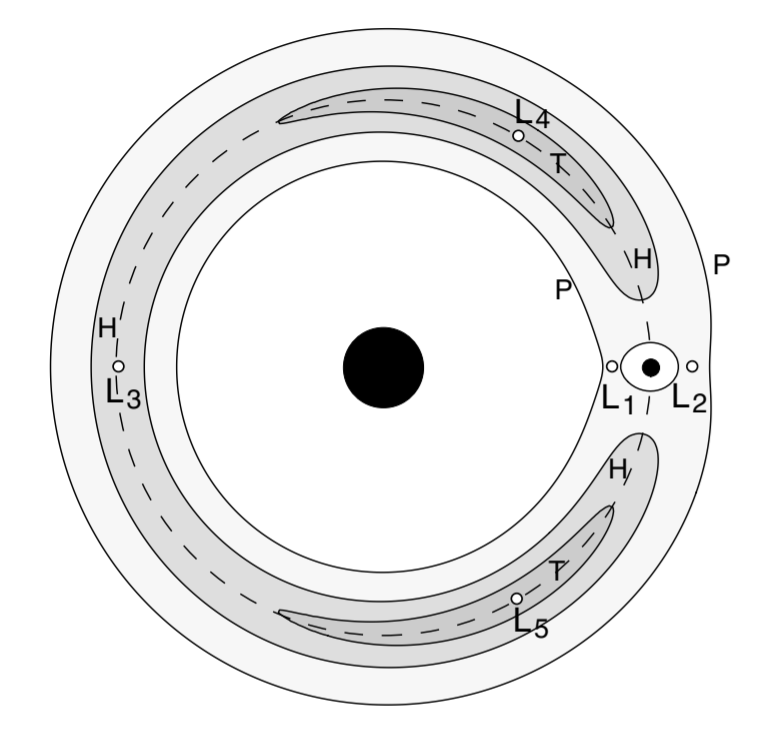
\includegraphics[width=\linewidth]{Figures/lagrange_points}
	\caption{The location of the five Lagrange equilibrium points in the circular-restricted three-body problem. The solar and planetary masses are denoted by the large and small filled circles, and the letters P, H, and T denote passing, horseshoe, and tadpole orbits respectively. Note that the two masses form an equilateral triangle with each of the L\subscript{4} and L\subscript{5} points. Reproduced from Marzari et al. \cite{Marzari2002}}
	\label{fig:lagrangepoints}
\end{figure}

Figure \ref{fig:lagrangepoints} depicts orbits about L\subscript{4} and L\subscript{5} (known as tadpole orbits), as well as orbits between Lagrange points are also possible (such as horseshoe orbits), described by Murray et al. \cite{Murray1999}.

This report will focus on tadpole orbits, a well documented feature of Trojan orbits \cite{Garfinkel1983}, \cite{Dermott1981}, and the restricted three-body problem in general. Their distinctive shape is result of a long-period motion about the equilibrium point combining with a short-period oscillation due to Keplerian motion of the asteroid.

Szebehely et al. \cite{Szebehely1969} predict this short period tends to the planetary period in the small planetary mass limit, while the long period is given by

\begin{equation}
T_{long} = T_{P} \sqrt{\frac{4}{27 \mu_{2}}},  
\end{equation}

where $\mu_{2} = m_{2} / (m_{1} + m_{2})$ and $ T_{P} $ is the period of planetary orbit.

\subsection{Theoretical Model} \label{theory}
The three body problem, where the dynamics of three interacting bodies are determined given their initial positions and velocities, has no analytical (closed-form) solution in the general case \cite{Barrow2008}.

In this report, I will consider the circular, restricted, three-body problem, where two of the bodies move in circular, coplanar orbits about their common centre of mass (CoM), unaffected by the negligible mass of the third body. I will also assume that all interactions are via Newtonian gravity.

The system of differential coordinates determine the position and velocity of the asteroids, with two equations per spatial coordinate.
\begin{equation}
\frac{dr_{i}}{dt} = v_{i}, \frac{dv_{i}}{dt} = g_{i}, \quad i = x,y 
\end{equation}

In this, $g_{i}$ is given by:
\begin{equation}
\textbf{g}= - \frac{G M_{s}}{\lvert \textbf{r} - \textbf{r}_{s} \rvert ^{3}} (\textbf{r} - \textbf{r}_{s})
		 - \frac{G M_{p}}{\lvert \textbf{r} - \textbf{r}_{p} \rvert ^{3}} (\textbf{r} - \textbf{r}_{p})
\end{equation}
where the subscripts \textit{s} and \textit{p} refer to solar and planetary properties respectively.

We may also consider a frame rotating at the same speed as the massive bodies. As there is 1:1 orbital resonance between Jupiter and the asteroids, all three bodies are stationary in this frame. This significantly increases the accuracy of numerical simulations, as the exact solution is stationary with no explicit time dependence, rather then requiring an infinite power series \cite{Guglielmi2001}, \cite{LeVeque2007}.

When transforming into this rotating non-inertial frame, $g_{i}$ gains an additional virtual force term with coupling between the spatial coordinates. This is given below as the sum of the centripetal and Coriolis forces:

\begin{equation}
\Delta g_{i} = \Omega^{2} r_{i} - 2[\bm{\Omega} \times \textbf{v}]_{i}
\end{equation}
where $\Omega$ is the angular speed of the rotating frame, and $\textbf{v}$ is the velocity of the asteroid within this frame. 


\subsection{Symmetry}
This problem contains a number of symmetries, which could be employed to simplify the problem and reduce the computational load. The Trojan and Greek asteroids are in equivalent positions, so experience the same forces, and the system is rotationally and inversion symmetric, so the choice of initial point and orbit direction is arbitrary. Therefore only the Greeks, orbiting counter-clockwise with perturbations applied at t = 0, need to be investigated.

\subsection{Orbit Geometry}
As the three bodies considered here form an equilateral triangle in the initial equilibrium state, as depicted in Figure \ref{fig:geometry}, we can derive the polar coordinates of each body with respect to the centre of mass about which the bodies orbit.

\begin{figure}
	\centering
	\resizebox{\columnwidth}{!}{%
		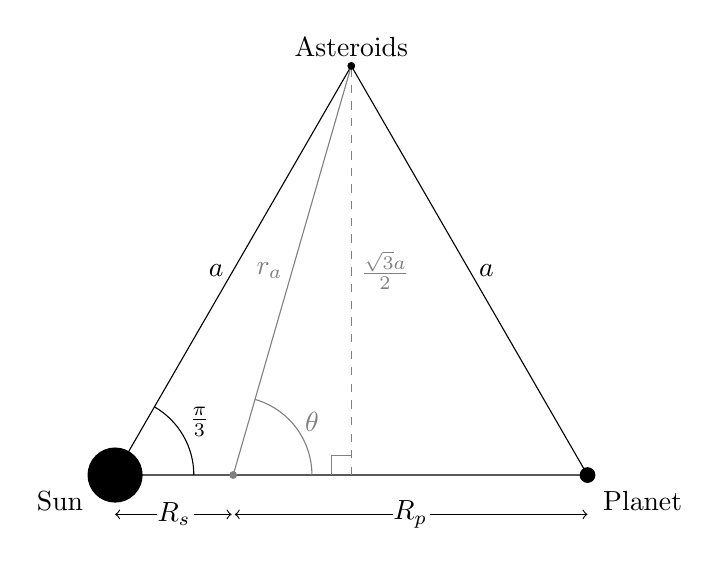
\begin{tikzpicture}
		\draw (0,0) -- (6,0) -- (3, {6*sin(60)} ) node[above]{Asteroids} node[midway,right]{$a$} -- cycle node[midway,left]{$a$};
		\draw  (1,0) arc (0:60:1cm)  ;
		%\node [label={[shift = {(10mm,5mm)}]{$\frac{\pi}{3}$}}] {};
		\node [label={[shift = {(13:11mm)}]{$\frac{\pi}{3}$}}] {};
		\node [label={[shift = {(-7mm,-7mm)}]{Sun}}] {};
		\node [label={[shift = {(67mm,-7mm)}]{Planet}}] {};
		
		\fill[gray] ({6*(1/4)}, 0) circle (0.5mm);
		\draw[gray] ({6*(1/4)}, 0) -- (3, {6*sin(60)} ) node[midway,left]{$r_{a}$};
		\draw[dashed, gray] (3, 0) -- (3, {6*sin(60)} )node[midway,right]{$\frac{\sqrt{3}a}{2}$};
		\draw[gray]  ({6*(1/4) + 1}, 0) arc (0:{atan(4*sin(60))}:1cm)  ;
		\node [label={[gray, shift = {(25mm,3mm)}]$\theta$}] {};
		\draw[gray] (2.75,0) -- (2.75, 0.25) -- (3, 0.25);
		
		\draw[arrows=<-](0,-0.5)--(0.53,-0.5);
		\node at (0.75, -0.5) {$R_s$};
		\draw[arrows=->](1.0,-0.5)--(1.48,-0.5);
		
		\draw[arrows=<-](1.52,-0.5)--(3.53,-0.5);
		\node at (3.75, -0.5) {$R_p$};
		\draw[arrows=->](4.00,-0.5)--(6,-0.5);
		
		%\draw[arrows=<-](0,-1)--(2.88,-1);
		%\node at (3, -1) {$a$};
		%\draw[arrows=->](3.1,-1)--(6, -1);
		
		\fill[black] (0,0) circle (3.5mm);% node[anchor=north west] {Sun};
		\fill[black] (6,0) circle (1mm);
		\fill[black] (3, {6*sin(60)} ) circle (0.5mm);
		
		\end{tikzpicture}
	}	
	\caption{A geometric depiction of the three-body system, in the case where the planet has a mass equal to a third of the sun, and asteroids are considered at the L\subscript{4} point. $ R_{s} $ and $ R_{p}$ denote the (fixed) radii from the centre of mass (the grey point) to the Sun and the planet respectively, while $ r_{a} $ denotes the radius of the asteroids.}
	\label{fig:geometry}
\end{figure}

Using standard trigonometric relations, it is simple to show that the values $ r_{a} $ and $ \theta $ are given by:

\begin{equation}
r_{a} = \sqrt{a^{2} + R_{s} R_{p}} , \enspace \theta =  \tan^{-1} \left( \frac{a \sin(\frac{\pi}{3})}{R_{p} - \frac{a}{2}} \right)
\end{equation}

Furthermore, the Lagrange point in Cartesian coordinates based about the CoM is easily found to be:

\begin{equation}
(x,y) = \left( R_{p} - \frac{a}{2}, \frac{ \sqrt{3} a}{2} \right)
\end{equation}

Finally, equating the gravitational and centripetal forces on the planet allows the derivation of its (and all other bodies') orbital velocity:

\begin{equation}
\Omega = \sqrt{\frac{G (M_{s} + M_{p})}{a^{3}}}
\end{equation}

\section{Methodology}
This system of coupled first-order ordinary differential equations (ODEs) was solved using the scipy solve\_ivp function. The time span was taken as 100 orbits (with 100 points sampled per orbit) unless otherwise stated; this corresponds to 1185 Earth years. Rescaled solar system units are used for mathematical ease, so distances are measured in astronomical units (AU), time in earth years and mass in multiples of the solar mass, and to prevent floating point overflows due to the magnitude of the quantities considered in SI units.

The wander was defined as the maximum distance of the asteroid from the initial point during the orbit (for small perturbations this is also approximately the separation from the Lagrange point).
Initial conditions are defined by the Lagrange point in each frame, with the initial velocity in the stationary frame defined by the period of Jupiter's orbit, and split into Cartesian components.

\subsection{Integration Method}
%Put this with theory as "numerical methods"?
%Then all theory could be in methodology?
Within solve\_ivp, the default solver is RK45 (an explicit Runge-Kutta method of order 5(4) \cite{Dormand1980}) and gives a deviation in asteroid position (from the Lagrange point) in the order of $ 10^{-4}$ AU in the rotating frame over 50 years. This is larger than expected, indicating the system of equations requires an unreasonably small step size for numerical stability with respect to this method, even in regions where the solution curve is smooth \cite{Lambert1991}. This suggests the system is stiff, and solvers designed for this typically do more work per step, allowing them to take much larger steps, and have improved numerical stability compared to the non-stiff solvers such as RK45 \cite{Byrne1987}. 

Instead the stiff "Radau" solver (an implicit Runge-Kutta method of the Radau IIA family of order 5 \cite{Hairer2010}) is used for increased stability \cite{Frank1985}, and achieves a deviation in asteroid position in the order of $ 10^{-13}$ AU instead. This also ensures stability in the stationary frame, with deviations of 0.76\% in asteroid separation from Jupiter over $ 10^{3} $ years, compared to 53\% for the best non-stiff solvers.

%Can add more detail on A vs B stability (I believe B stability is relevant here but maybe check this)

\subsection{Programme Structure}
Global constants such as solar mass, and sun\textendash planet separation, along with derived values from these such as orbital period and solar radius from the CoM, are given in an importable python module "\textit{constants}".

Functions to evaluate these coupled differential equation systems are defined in module "\textit{orbits}", while additional functions to evaluate the wander during the orbit (under different sampling routines) are implemented in "\textit{wander}". Further files then import these modules and produce the plots given in this report, fully detailed in appendix \ref{structure}.

To consider a varying planet mass, it was considered preferable to avoid reconstructing all functions to take this as an argument as this requires re-evaluating all initial derived constants. Therefore, I iterate over alternative masses, re-defining constant values in this instance, and then directly import the required functions to compute the orbit. \textbf{REPHRASE?}

Complete code listings are given in appendix \ref{Code}.


\subsection{Performance} \label{Performance}
Sampling 100 points per orbit for 100 orbits takes a mean time of $16.97 \pm 34$ \si{\milli\second}, with sub-linear scaling for sampling rate and orbit number up to the array memory limit, achieved through the optimised integration routines within solve\_ivp.


\section{Results}
\subsection{Unperturbed Stability of Lagrange Points} \label{unperturbed}
Considering the Greeks' orbit without perturbations applied, it has a maximum deviation of $4.68 \times 10^{-13}$ AU over 100 orbits (1185 years). This value is unchanged if 1000 orbits are considered instead, confirming the stability of this Lagrange point.

In the stationary frame, this wander from the (now moving) Lagrange point is depicted in Figure \ref{fig:greeksdeviationstationaryframe}. The deviation oscillates with a magnitude of $9.10 \times 10^{-2}$ AU, and a period of $148 \pm 4$ years, where the error was determined by the width of the Fourier peak. This is modulated with a faster oscillation component of $11.85 \pm 0.27$ years, equivalent to the orbital period of the asteroids.

\begin{figure}
	\centering
	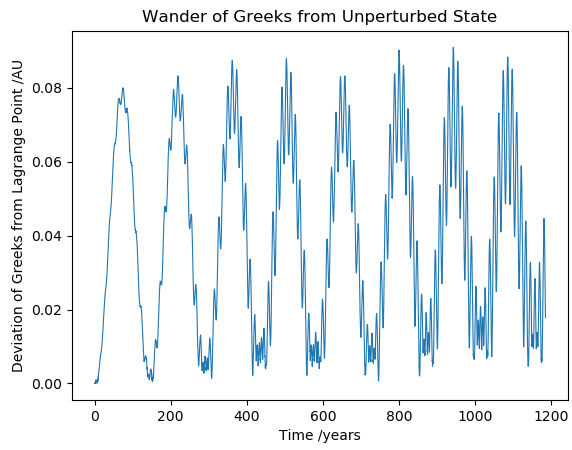
\includegraphics[width=\linewidth]{Figures/greeks_deviation_stationary_frame}
	\caption{The wander of Greek asteroids from the Lagrange point in the stationary frame. Note the two oscillation components and constant maximum oscillation amplitude over time, demonstrating this point is indeed stable.}
	\label{fig:greeksdeviationstationaryframe}
\end{figure}

These much more significant errors are due to time dependence in the exact solution, as detailed in Section \ref{theory}. Energy can also be evaluated, and conserved, in this inertial frame; asteroid specific energy varies within only 0.113\% of the initial value, and with a similar periodicity to wander. Energy is also negative, confirming the asteroids are located within a bound orbit.

Animations produced to demonstrate the orbit in the stationary frame are included in Supplementary Material I-II. Animation I depicts the orbit as evaluated by the radau solver, while II depicts it with LSODA, demonstrating the drift present over time with non-stiff solvers.

\subsection{Wander Analysis} \label{perturbed}
The wander from the initial point was calculated for random perturbations with a maximum magnitude of 1\% of the displacement from the origin, and considered  separately perturbation components parallel and perpendicular to the position vector from the CoM (hereafter referred to as radial and tangential components respectively). By considering these perturbations across position space, it was clear that the wander is fully determined by the radial component, with no tangential dependence (as shown in Figure \ref{fig:wanderplots}).


\begin{figure}[ht]
	\centering
	\begin{subfigure}{.45\textwidth}
		\centering
		% include first image
		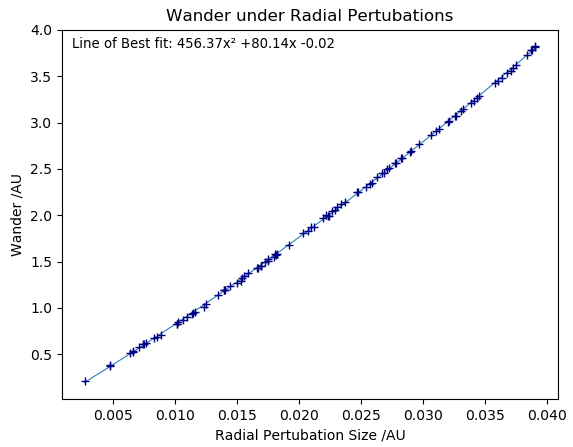
\includegraphics[width=\linewidth]{Figures/wanderagainstradialpertubation2}  
		\caption{Radial}
		\label{fig:wander_rad}
	\end{subfigure}
	\hfill %% useful if width of each figure is less the .5\textwidth
	\begin{subfigure}{.45\textwidth}
		\centering
		% include second image
		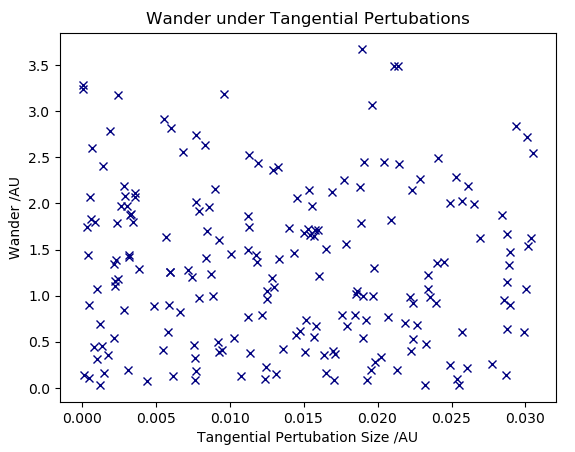
\includegraphics[width=\linewidth]{Figures/wanderagainsttangentialpertubation2}  
		\caption{Tangential}
		\label{fig:wander_tan}
	\end{subfigure}
	\caption{Wander from an initial perturbation with maximum relative magnitude of 0.1\% of the displacement from the origin, given in radial and tangential directions.}
	\label{fig:wanderplots}
\end{figure}

Figure \ref{fig:wander_rad} demonstrates a polynomial dependence on perturbation size in the radial direction, with a negligible constant term. While a quadratic has been fitted here, it was not possible to eliminate the possibility of higher order terms, as increasing perturbation size beyond 0.06 AU can lead to unstable orbits.

We may consider the wander resulting from perturbations in position and velocity space. Figure \ref{fig:position_mesh} clearly shows the dependence on radial position perturbations only, while Figure \ref{fig:velocity_mesh} shows a similar the dependence on tangential velocity perturbations.

\begin{figure}[ht]
	\centering
	\begin{subfigure}{.45\textwidth}
		\centering
		% include first image
		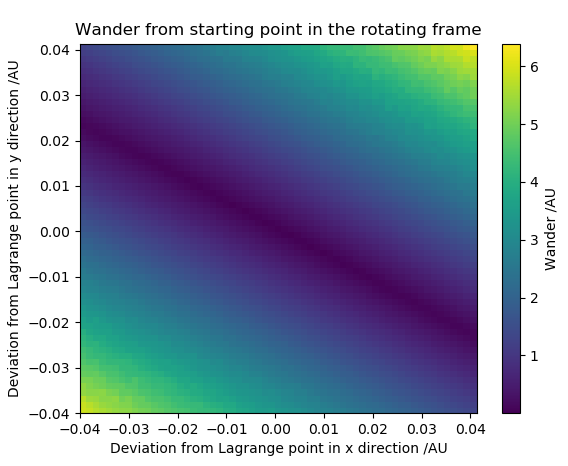
\includegraphics[width=\linewidth]{Figures/testcolourmesh6}  
		\caption{Position}
		\label{fig:position_mesh}
	\end{subfigure}
	\hfill %% useful if width of each figure is less the .5\textwidth
	\begin{subfigure}{.45\textwidth}
		\centering
		% include second image
		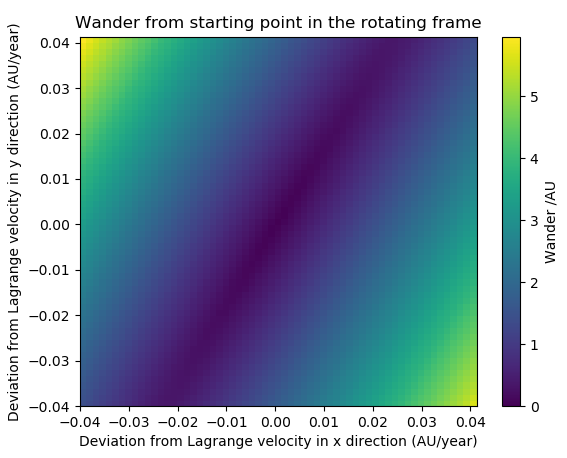
\includegraphics[width=\linewidth]{Figures/testvelocitymesh2}  
		\caption{Velocity}
		\label{fig:velocity_mesh}
	\end{subfigure}
	\caption{Wander from an initial point in position and velocity space, only calculated over 50 orbits with 30 points per orbit to reduce computational load. Note the dependence on radial position and tangential velocity perturbation components. }
	\label{fig:mesh_plots}
\end{figure}

\subsection{Orbit Types} \label{orbits}
Figure \ref{fig:orbitplots} displays orbits resulting from small perturbations in the radial and tangential directions.

\begin{figure}[ht]
	\centering
	\begin{subfigure}{.23\textwidth}
		\centering
		% include first image
		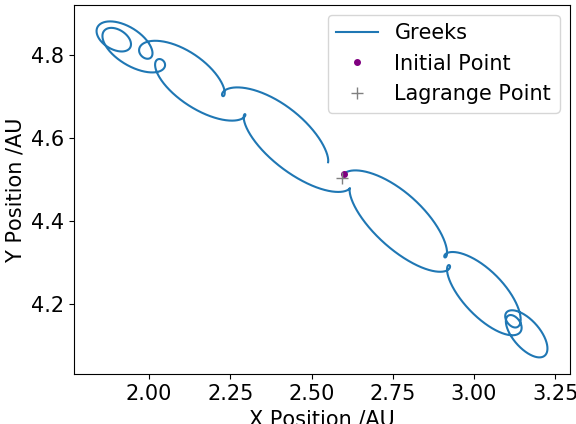
\includegraphics[width=\linewidth]{Figures/radialp_orbits}  
		\caption{Radial}
		\label{fig:orbit_rad}
	\end{subfigure}
	\hfill %% useful if width of each figure is less the .5\textwidth
	\begin{subfigure}{.23\textwidth}
		\centering
		% include second image
		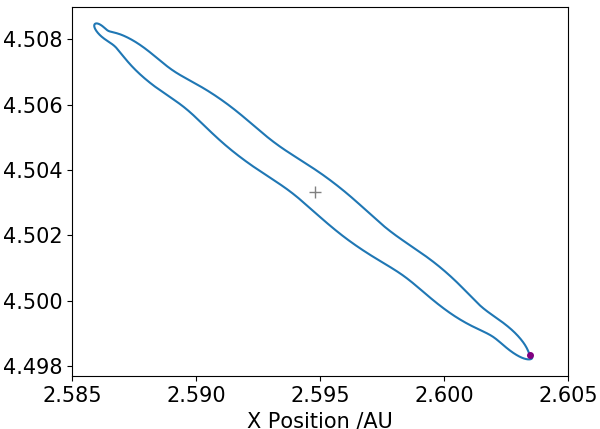
\includegraphics[width=\linewidth]{Figures/tangentialp_orbits}  
		\caption{Tangential}
		\label{fig:orbit_tan}
	\end{subfigure}
	\caption{Orbits from an initial perturbation of magnitude 0.01 AU from the origin, in radial and tangential directions, over 12 orbital periods. Note the 'tadpole' features resulting from the radial perturbation, and the significantly larger wander than from the tangential perturbation.}
	\label{fig:orbitplots}
\end{figure}


 
The "tadpole" orbit in Figure \ref{fig:orbit_rad} consists of two oscillating components, as described in Section \ref{lagrange}. The short period, measured at $11.85 \pm 0.61$ years, is in excellent agreement with  planetary orbital period as expected; meanwhile the long period is measured to be $148 \pm 5$ years, consistent with the analytical value of $144$ years.

For a narrow range of larger perturbations, stable horseshoe orbits encompassing both Lagrange points may also be observed as depicted in Figure \ref{fig:horseshoe}. This has a full period of $353$ years, in agreement with Taylor et al.'s numerical result of $358 \pm 7$ years \cite{Taylor1981}.

%smooth families of horseshoe-shaped longperiodic orbits for alpha2 > 1. Smooth, because they are restricted to shallow resonance, where the evolution of the epicyclic cusps and loops cannot be seen. - according to taylor, but havn't found smooth orbits here

\begin{figure}
	\centering
	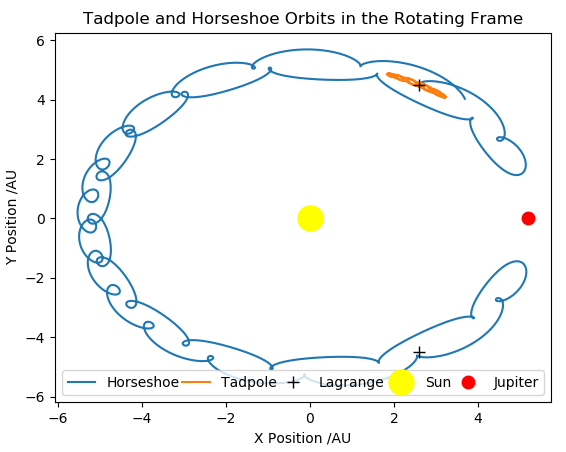
\includegraphics[width=0.8\linewidth]{Figures/horseshoe}
	\caption{Horseshoe and tadpole orbits in the rotating frame, from radial perturbations of 0.07 and 0.01 AU respectively, over 30 orbital periods.}
	\label{fig:horseshoe}
\end{figure}

\subsection{Perturbations in z-direction} \label{3D}

\subsection{Variation of Planetary Mass} \label{planet}
The variation of wander with planetary mass is given in Figure \ref{fig:planetmass}.

\begin{figure}
	\centering
	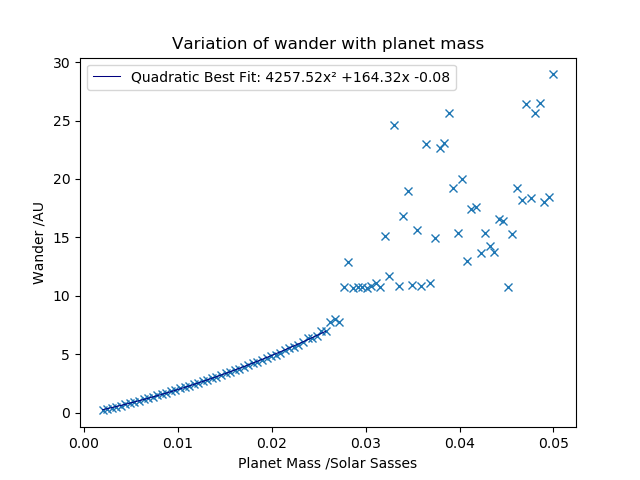
\includegraphics[width=0.8\linewidth]{Figures/wanderwithplanetmass_p5b}
	\caption{Variation of maximum wander with planetary mass. Note the well defined quadratic trend up to $ M_{p} = 0.026 M_{s}$, and instability beyond this.}
	\label{fig:planetmass}
\end{figure}

A quadratic trend (with a large quadratic component) is initially observed, but wander deviates from this at approximately $ M_{p} = 0.026 M_{s}$, with a sharp increase indicating orbit instability. This occurs significantly before the theoretical prediction of $ M_{p} = 0.04 M_{s}$ \cite{Darwin1897}, however it is suggested this is due to instabilities in the integration solver.

\section{Conclusion}




\clearpage
\printbibliography

\onecolumn
\begin{appendices}
\section{Program Structure} \label{structure}
Global constants, along with derived values from these are given in an python module "\textit{constants}", from which relevant variable are imported in all other scripts.

Functions to evaluate these coupled differential equation systems are defined in module "\textit{orbits}", while additional functions to evaluate the wander during the orbit are implemented in "\textit{wander}". These modules are both imported into the scripts below for plotting and analysis, and given in the listings in Appendix \ref{Code}.

\textit{Wander from unperturbed initial conditions is calculated within "\textit{lagrange\_stability}", with ODE solver performance also evaluated here.
Orbits in the stationary frame are animated and saved within "\textit{stat\_frame\_video}".

2D perturbations are characterised in \textit{perturbation\_2D}, while perturbations in the z direction are considered in \textit{perturbation\_3D}. Variation in planetary mass, for results in section \ref{planet}, are given in \textit{planet\_mass\_variation}.}

Other code files are listed by Section below in Table \ref{Codefiles}:

\begin{table}[ht]
	\caption{Program files used to generate results in each section, with a description of their role.}
	\centering
	\begin{tabular}{|c|c|c|}
		\hline
		\textbf{Section} & \textbf{Description} & \textbf{Code File} \\
		\hline \hline
		\ref{Performance} & ODE solver performance & \textit{lagrange\_stability} \\
		\hline
		\ref{unperturbed} & Wander from unperturbed initial conditions & \textit{lagrange\_stability} \\
		\hline
		\ref{unperturbed} & Animations of unperturbed orbits & \textit{stat\_frame\_video} \\
		\hline
		\ref{perturbed}& Perturbations restricted to the xy plane & \textit{perturbation\_2D} \\
		\hline
		\ref{orbits}& Plotting of Orbit types in xy plane & \textit{perturbation\_2D} \\
		\hline
		\ref{3D}& Perturbations in the z-direction & \textit{perturbation\_3D} \\
		\hline
		\ref{planet}& Variation of planetary mass & \textit{planet\_mass\_variation} \\
		\hline
	\end{tabular}
	\label{Codefiles}
\end{table}


\section{Code Listings} \label{Code}
\begin{lstlisting}[language=Python]
import math
import numpy as np
from scipy import integrate
import matplotlib.pyplot as plt

from constants import G, M_S, M_P, R, ORBIT_NUM, PRECISION  # User defined constants
from constants import (
	solar_rad,
	planet_rad,
	period,
	omega,
	time_span,
)  # Derived constants


\end{lstlisting}
%Can add my own style guide to this, see suggestions on https://www.overleaf.com/learn/latex/code_listing
%\section{Code 2}

\end{appendices}

\end{document}

%%%%%%%%%%%%%%%%%%%%%%%%%%%%%%%%%%%%%%%%%
% Wenneker Article
% LaTeX Template
% Version 2.0 (28/2/17)
%
% This template was downloaded from:
% http://www.LaTeXTemplates.com
%
% Authors:
% Vel (vel@LaTeXTemplates.com)
% Frits Wenneker
%
% License:
% CC BY-NC-SA 3.0 (http://creativecommons.org/licenses/by-nc-sa/3.0/)
%
%%%%%%%%%%%%%%%%%%%%%%%%%%%%%%%%%%%%%%%%%
